%%%%%%%%%%%%%%%%%%%%%%%%%%%%%%%%%%%%%%%%%
% Jacobs Landscape Poster
% LaTeX Template
% Version 1.1 (14/06/14)
%
% Created by:
% Computational Physics and Biophysics Group, Jacobs University
% https://teamwork.jacobs-university.de:8443/confluence/display/CoPandBiG/LaTeX+Poster
% 
% Further modified by:
% Nathaniel Johnston (nathaniel@njohnston.ca)
%
% This template has been downloaded from:
% http://www.LaTeXTemplates.com
%
% License:
% CC BY-NC-SA 3.0 (http://creativecommons.org/licenses/by-nc-sa/3.0/)
%
%%%%%%%%%%%%%%%%%%%%%%%%%%%%%%%%%%%%%%%%%

%----------------------------------------------------------------------------------------
%	PACKAGES AND OTHER DOCUMENT CONFIGURATIONS
%----------------------------------------------------------------------------------------

\documentclass[final]{beamer}

\usepackage[scale=1.0]{beamerposter} % Use the beamerposter package for laying out the poster
\usetheme{confposter} % Use the confposter theme supplied with this template

\setbeamercolor{block title}{fg=dblue!80,bg=white} % Colors of the block titles
\setbeamercolor{block body}{fg=black,bg=white} % Colors of the body of blocks
\setbeamercolor{block alerted title}{fg=white,bg=dblue!70} % Colors of the highlighted block titles
\setbeamercolor{block alerted body}{fg=black,bg=dblue!10} % Colors of the body of highlighted blocks
% Many more colors are available for use in beamerthemeconfposter.sty

%-----------------------------------------------------------
% Define the column widths and overall poster size
% To set effective sepwid, onecolwid and twocolwid values, first choose how many columns you want and how much separation you want between columns
% In this template, the separation width chosen is 0.024 of the paper width and a 4-column layout
% onecolwid should therefore be (1-(# of columns+1)*sepwid)/# of columns e.g. (1-(4+1)*0.024)/4 = 0.22
% onecolwid should therefore be (1-(# of columns+1)*sepwid)/# of columns e.g. 
% (1-(3+1)*0.025)/3 = 0.3
% Set twocolwid to be (2*onecolwid)+sepwid = 0.464
% Set threecolwid to be (3*onecolwid)+2*sepwid = 0.708

\newlength{\sepwid}
\newlength{\onecolwid}
\newlength{\twocolwid}
\newlength{\threecolwid}
\setlength{\paperwidth}{36in} % A0 width: 46.8in
\setlength{\paperheight}{48in} % A0 height: 33.1in
\setlength{\textwidth}{34in} % A0 width: 46.8in
\setlength{\textheight}{46in} % A0 height: 33.1in
\setlength{\sepwid}{0.025\paperwidth} % Separation width (white space) between columns
\setlength{\onecolwid}{0.3\paperwidth} % Width of one column
\setlength{\twocolwid}{0.625\paperwidth} % Width of two columns
\setlength{\threecolwid}{0.95\paperwidth} % Width of three columns
\setlength{\topmargin}{-0.5in} % Reduce the top margin size
%-----------------------------------------------------------

\usepackage{graphicx}  % Required for including images
\newcommand{\Cyclus}{\textsc{Cyclus}\xspace}%

\usepackage{tabularx}
\newcolumntype{b}{X}
\newcolumntype{s}{>{\hsize=.5\hsize}X}
\newcolumntype{m}{>{\hsize=.75\hsize}X}
\newcolumntype{z}{>{\hsize=.65\hsize}X}

\usepackage{booktabs} % Top and bottom rules for tables
\usepackage{xspace}

\usepackage{tikz}
\usetikzlibrary{positioning, arrows, decorations, shapes, arrows.meta}
% Define block styles
\tikzstyle{decision} = [diamond, draw, fill=blue!20, 
text width=4.5em, text badly centered, node distance=3cm, inner sep=0pt]


\tikzstyle{block} = [rectangle, draw, text centered, fill=blue!20]
\tikzstyle{line} = [draw, -latex']
\tikzstyle{cloud} = [draw, ellipse,fill=red!20, node distance=6em,
minimum height=2em]



\usetikzlibrary{shapes.multipart}
\usetikzlibrary{positioning}


\setbeamertemplate{bibliography item}[text]

%----------------------------------------------------------------------------------------
%	TITLE SECTION 
%----------------------------------------------------------------------------------------

\title{
	
\includegraphics[width=0.2\linewidth]{ilogo}
	\hspace{30cm}
	\vspace{2cm}
	
\includegraphics[width=0.3\linewidth]{cnec_logo} \\
	Diversion Detection in Cyclus Archetpyes
} % Poster title

\author{\textbf{Gregory T. Westphal}, Kathryn D. Huff}
\institute{University of Illinois at Urbana-Champaign, Department of Nuclear, Plasma, and Radiological Engineering, Urbana, IL 61801}
%----------------------------------------------------------------------------------------

\begin{document}

\addtobeamertemplate{block end}{}{\vspace*{2ex}} % White space under blocks
\addtobeamertemplate{block alerted end}{}{\vspace*{2ex}} % White space under highlighted (alert) blocks

\setlength{\belowcaptionskip}{2ex} % White space under figures
\setlength\belowdisplayshortskip{2ex} % White space under equations

\begin{frame}[t] % The whole poster is enclosed in one beamer frame

\begin{columns}[t,totalwidth=\threecolwid] % The whole poster consists of three major columns, the second of which is split into two columns twice - the [t] option aligns each column's content to the top

\begin{column}{0.5\sepwid}\end{column} % Empty spacer column

\begin{column}{\onecolwid} % The first column

%----------------------------------------------------------------------------------------
%	OBJECTIVES
%----------------------------------------------------------------------------------------

\begin{alertblock}{Objectives}
\begin{itemize}
        \item Timely detection of diversion relies on the identification of signatures and observables for unique facilities. 
        \item Create high-fidelity diversion algorithms.
        \item Determine optimum detector and inspection locations in pyroprocessing facilities using the Cyclus framework.
        \item Adapt this work to be applicable to a wide range of nuclear fuel cycle facilities in Cyclus
        \item Characterize required detection sensitivities and corresponding 
                false positive rates. 
\end{itemize}

\end{alertblock}

%----------------------------------------------------------------------------------------
%	BACKGROUND
%----------------------------------------------------------------------------------------

\begin{block}{Background}


\begin{figure}
	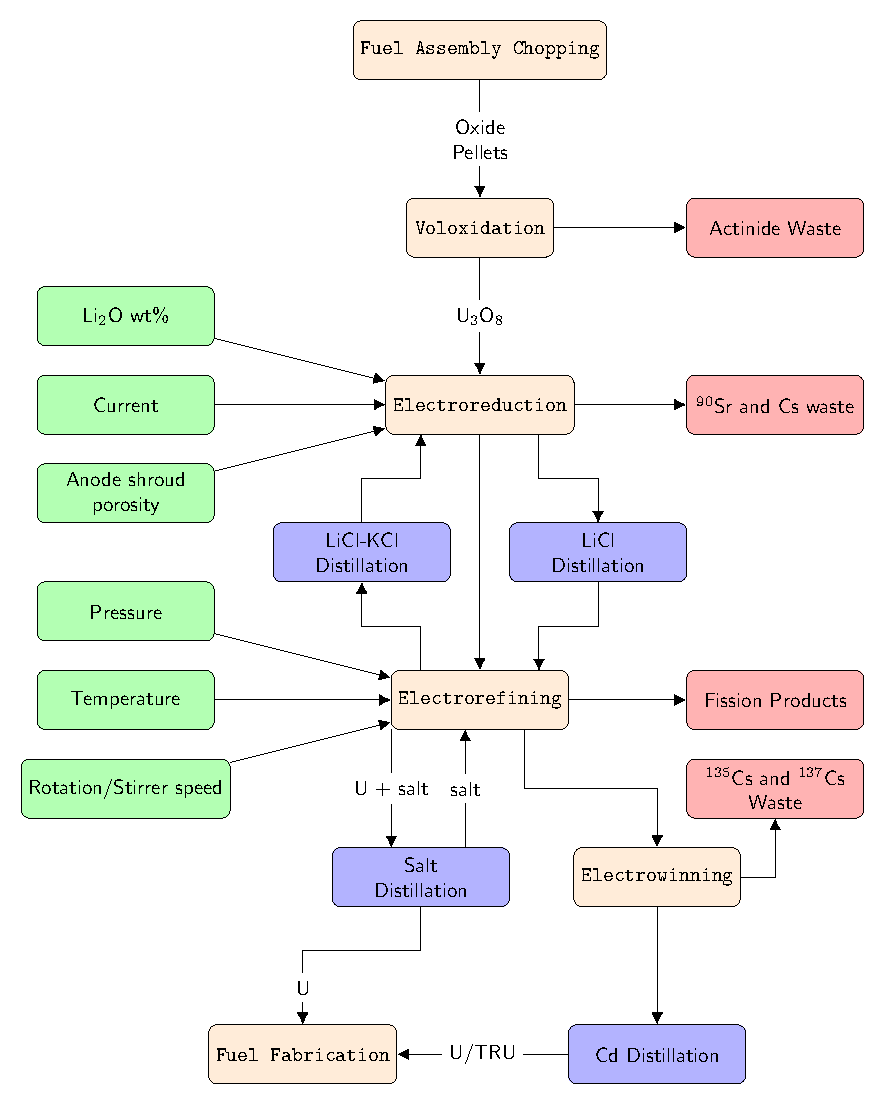
\includegraphics[width=\linewidth]{flowchart.pdf}
%	\includegraphics[width=1.0\linewidth]{fuel_cycle2.png}
        %\input{fc-diagram}
	\caption{Archetpye design of the Pyre facility \cite{Borrelli_2017}.}
\end{figure}

\end{block}

%----------------------------------------------------------------------------------------
%	DIVERSION DETECTION
%----------------------------------------------------------------------------------------

\begin{block}{Facility Simulation}

	\begin{figure}
		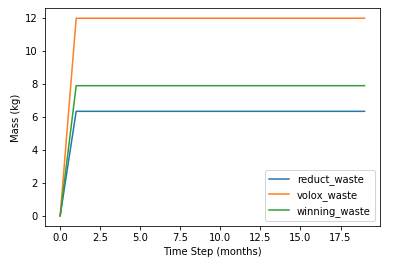
\includegraphics[width=0.9\linewidth]{timeseries-waste.png}
		\caption{Example material transactions every time step.}
	\end{figure}

	\begin{figure}
		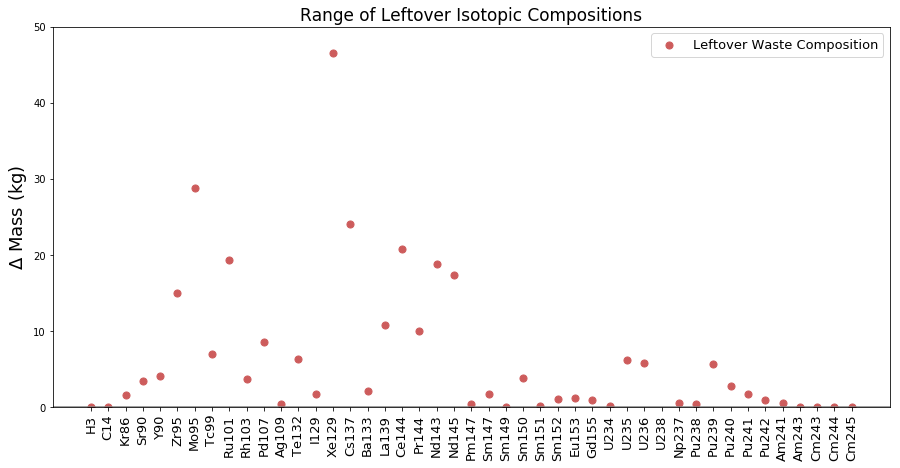
\includegraphics[width=0.9\linewidth]{isotopic-comp-range.png}
		\caption{The isotopic breakdown of material transactions in the facility.}
	\end{figure}
\end{block}

%----------------------------------------------------------------------------------------

\end{column} % End of the first column

\begin{column}{\sepwid}\end{column} % Empty spacer column


%----------------------------------------------------------------------------------------

\begin{column}{\onecolwid} % The second column
%----------------------------------------------------------------------------------------
%	SIGNATURES AND OBSERVABLES
%----------------------------------------------------------------------------------------

\begin{block}{Material Diversion}
        Material diversion occurs in two different modes: \textbf{nefarious} or \textbf{operator}.
        \begin{itemize}
        \item \textbf{Nefarious Diversion} imagines diversion by a single bad actor with facility access.
        \item \textbf{Operator Diversion} imagines undeclared production.
        \item Either can be achieved by increasing plant throughput and siphoning off material excess for unsanctioned weapons production.
        \end{itemize}
        
        
	\begin{block} {Nefarious Diversion}
		\begin{figure}
			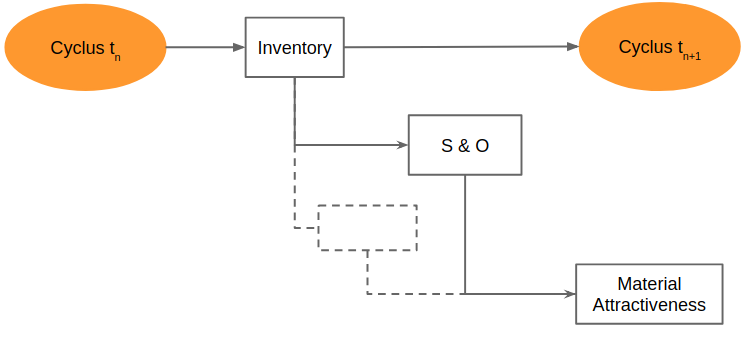
\includegraphics[width=0.9\linewidth]{diversion1.png}
			\caption{Illustration of nefarious diversion of Cyclus inventory.}
		\end{figure}
		
	\end{block}
	\begin{block} {Operator Diversion}
		\begin{figure}
			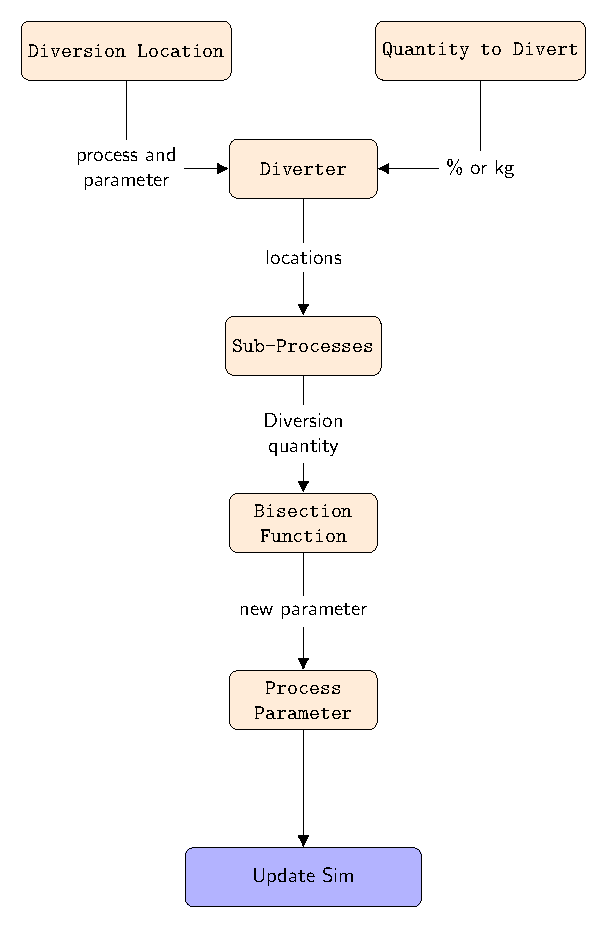
\includegraphics[width=0.8\linewidth]{op-diversion}
			\caption{Procedure for generating operator diversion values inside a simulation.}
		\end{figure}
		\begin{figure}
			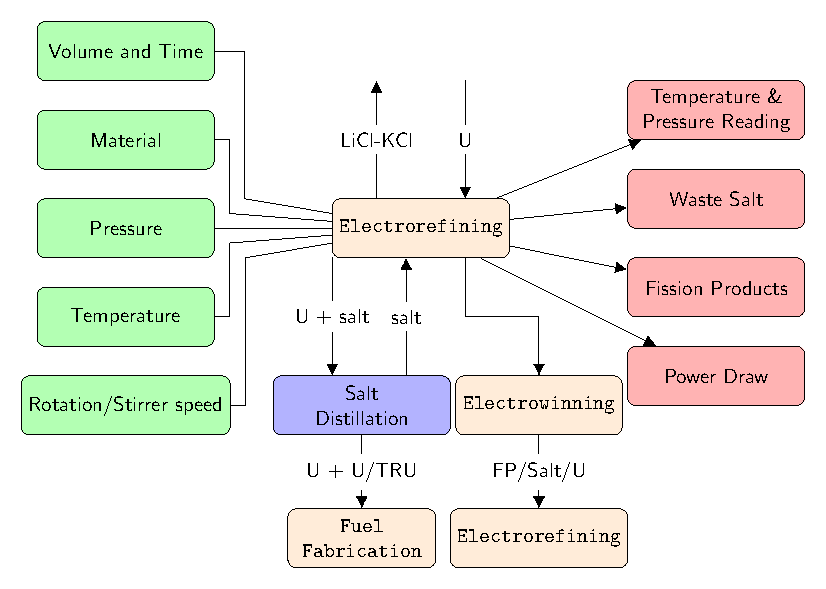
\includegraphics[width=\linewidth]{refining}
			\caption{Example material balance used over a sub-process for diversion detection \cite{lee_advanced_2008}.}
		\end{figure}
	\end{block}

\begin{center}
	\begin{tabular}{ccc}
		\centering
		
\includegraphics[width=0.45\linewidth]{nnsa}
	\end{tabular}
\end{center}
\end{block}
%----------------------------------------------------------------------------------------

\end{column} % End of column 2

\begin{column}{\sepwid}\end{column} % Empty spacer column

\begin{column}{\onecolwid} % The third column
	
\begin{block}{Diversion Detection}
	To maintain customization of the archetype a CUMUFR (cumulative sum of MUF residuals) algorithm is used.
	This approach has the benefit of not requiring a known mean value, however, time is required for the statistic before being able to accurately detect material diversion.
	\begin{figure}
		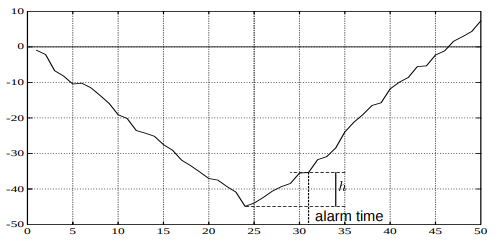
\includegraphics[width=0.9\linewidth]{cusum-example.png}
		\caption{Cumulative sum method being used to detect a change in material flow \cite{basseville_detection_1993}.}
	\end{figure}
	
\end{block}
%----------------------------------------------------------------------------------------
%	FUTURE WORK
%----------------------------------------------------------------------------------------
\begin{block}{Accomplishments}
	\begin{itemize}
		\item Created a highly customizable pyroprocessing facility within Cyclus.
		\item Performed a variety of "standard operation" simulations without diversion.
		\item Developed a method to handle multiple diversion modes and improve reproducibility.
	\end{itemize}
\end{block}

\begin{alertblock}{Future Work}
	\begin{itemize}
		\item Sensitivity analysis of diversion methods.
		\item Compare Cyclus output for various facility configurations.
		\item Assess capability of using Cyclus as online detection.
	\end{itemize} 
	\vspace{10mm}
	In addition to completing the diversion detection module for pyroprocessing, the goal is to expand this to be accessible to
	other Cyclus archetypes as well \cite{Huff_2016}. Other capabilities to be added include accounting for a variety of diversion times,
	currently the algorithm is capable of routine and set times for diversion.
\end{alertblock}

%----------------------------------------------------------------------------------------
%	ACKNOWLEDGEMENTS
%----------------------------------------------------------------------------------------

\setbeamercolor{block title}{fg=norange,bg=white} % Change the block title color

\begin{block}{Acknowledgements}
	
	This material is based upon work supported by
	the Department of Energy National Nuclear Security
	Administration under Award Number(s) DE-NA0002576 via
	the Consortium for Nonproliferation Enabling Capabilities.
	
	\vspace{10mm}
	\begin{center}
		\begin{tabular}{ccc}
			
\includegraphics[width=0.3\linewidth]{logo.png} & 
\includegraphics[width=0.5\linewidth]{cnec_logo}
		\end{tabular}
	\end{center}
	
	
\end{block}

%----------------------------------------------------------------------------------------
%	CONTACT INFORMATION
%----------------------------------------------------------------------------------------

\setbeamercolor{block alerted title}{fg=black,bg=norange} % Change the alert block title colors
\setbeamercolor{block alerted body}{fg=black,bg=white} % Change the alert block body colors



\begin{alertblock}{Contact Information}
	\setbeamercolor{block title}{fg=norange,bg=white} % Change the block title color
	\begin{itemize}
		
		\item Web: \href{arfc.github.io}{arfc.github.io}
		\item Email: \href{mailto:gtw2@illinois.edu}{gtw2@illinois.edu}
		\item Phone: +1 (636) 284-9691
	\end{itemize}
	
\end{alertblock}

\begin{block}{References}

        {\footnotesize\bibliographystyle{abbrv} 
        \bibliography{poster}}
\end{block}


%----------------------------------------------------------------------------------------



\end{column} % End of the third column

\end{columns} % End of all the columns in the poster

\end{frame} % End of the enclosing frame

\end{document}
\begin{column}{\sepwid}\end{column} % Empty spacer column
